\chapter{Introduction of E-I balanced Network and Point Attractor Network}\label{cpt:introduction}

\section{E-I balanced Network}
% brian persistent activity
Working memory in the brain can be interpreted as a persistent brain neuron activity even in the absence of an external stimulus.

It is found that population connection with positive and negative feedback or hybrid connection can lead to a persistent activity with a given pulse input into the neuron population.

The neuron populations with excitatory connections (both to itself and to other populations) are named as E neuron populations which will excite the following connected neuron, and the neuron populations with inhibitory connections are named as I neuron populations which will inhibit the following connected neuron. A model that is used for explain the persistent activities is shown in figure \ref{fig:reading_ei_persistant}.

% positive / negative feedback / derivative-feedback model
A self-positive excitation of E population is considered as positive feedback ($J_{EE}$) and 
the negative excitation of E population is considered as negative feedback($J_{II}$). 
The interconnection between E and I population is considered as shown in the figure \ref{fig:reading_ei_persistant} is considered as derivative feedback ($J_{EI}$)\cite{limBalancedCorticalMicrocircuitry2013}. 

% model behaivors
In this model, with pure positive feedback, the network can reach a persistent state, but it requires very careful parameter tuning and is not stable when external perturbance appears.

However, it is found that with a derivative feedback connection, the network can show the persistent activity by simply tuning the parameters and can be stable when external perturbance appears.

% EI balance and principle
This kind of network can be considered as a E-I balanced network. 

% analysis the principle maybe at last
%The principle behind this can be understand intuitively as: after E population perceiving an external input stimuli, it self-exciting its own population to help maintain the firing state (slowly). It also excites the I population, which instead inhibits the E population(fast). When the external stimuli is retreated, the inhibition disappears very fast

\begin{figure}
	\begin{subfigure}{.5\textwidth}
		\centering
		% include first image
		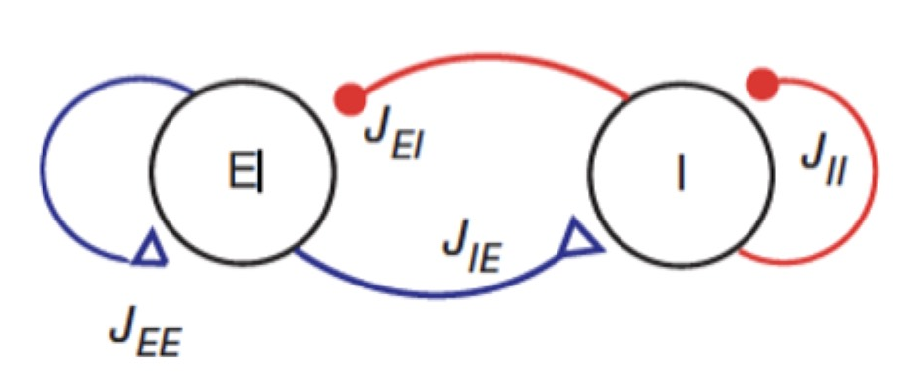
\includegraphics[width=\columnwidth]{./img/readings/EI_balance.pdf}
		\caption{The neuron population connection structure where the E population can realise a persistent activity.}
		\label{fig:ei_structure}
	\end{subfigure}
	\begin{subfigure}{.5\textwidth}
		\centering
		% include second image
		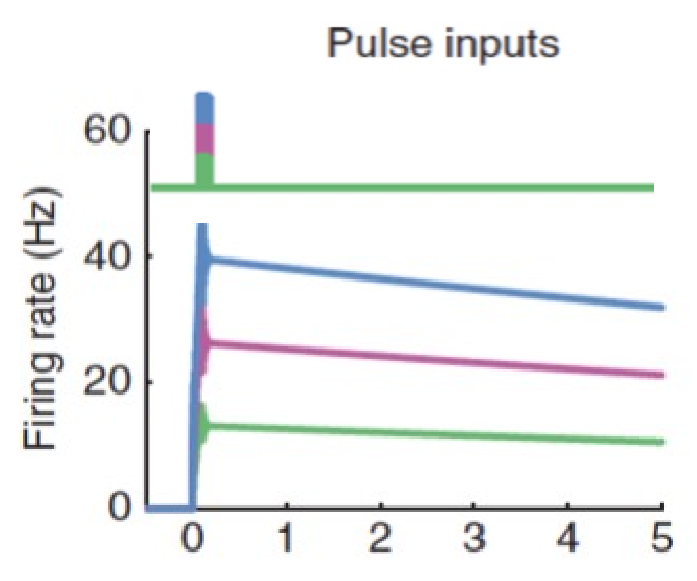
\includegraphics[width=\columnwidth]{./img/readings/persistent_activity.pdf}
		\caption{Persistent activity behaviour: given a pulse input, the neuron population will remain it's firing state for a longer period.}
		\label{fig:ei_persistent}
	\end{subfigure}
	\caption{The derivative network structure\cite{limBalancedCorticalMicrocircuitry2013} and persistent activity of a neuron population}
	\label{fig:reading_ei_persistant}
\end{figure}

\section{Point Attractor Network}
%Point Attractor Network
Besides the brief introduction of the theory of E-I balanced neural network, a VLSI neuromorphic chip is developed for emulating the neuronal behaviours. By connecting the neuron populations on this VLSI device, a E-I balanced network is realized which can implement a function as attracting the E population neurons to a persistent active state from a silent state by input excitatory stimuli. This active state is called an "attractor" state, and keep active even the external stimuli is removed. 
Since the network can stay at two stable states (one silent and one active),it  is named as a point attractor network. 
The point attractor network is self-correcting (which means it is robust to perturbation) and self-sustaining even without external stimulation \cite{giudiceRobustWorkingMemory2012}.

\subsection{Network structure}
\begin{figure}
	\centering
	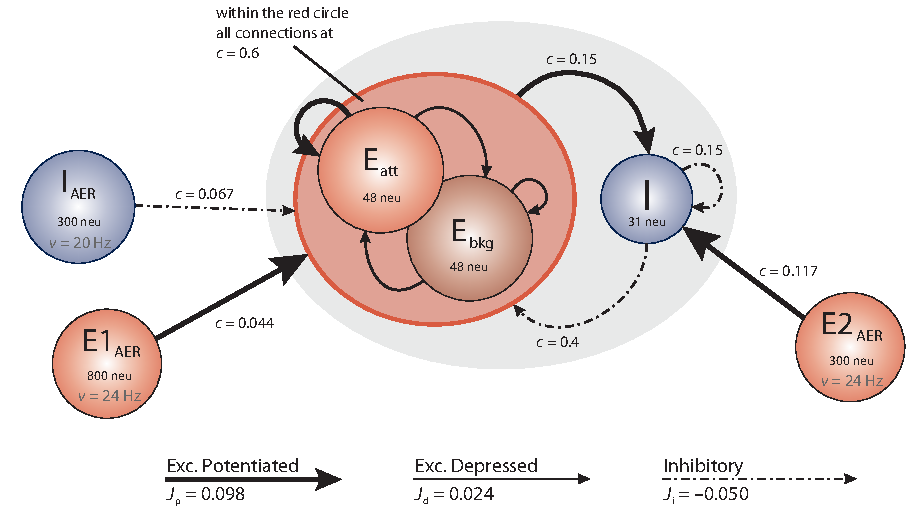
\includegraphics[width=\columnwidth]{./img/readings/WM_Network_structure.pdf}
	\caption{Network structure implemented on a VLSI chip to realize a point attractor network.}
	\label{fig:reading_NNonchip}
\end{figure}

% describe the connection
The architecture of the point attractor, which was implemented on a VLSI neuromorphic chip point attractor network is shown in figure \ref{fig:reading_NNonchip} \cite{giudiceRobustWorkingMemory2012}.

The excitatory population is divided into $E_{att}$ and $E_{bkg}$ populations, consisting of 48 neurons individually. The I population consists 31 neurons. 

The $E_{att}$ neurons are self-connected with excitatory potentiated synapses and $E_{bkg}$ neurons are self-connected with excitatory depressed synapses. $E_{bkg}$ and $E_{att}$ populations are inter-connected with a excitatory depressed synapse.
The excitatory potentiated synapse has a higher weight compared with excitatory depressed one. The E population connection probability is set as $c=0.6$.

The E population feeds forward its firing activity to I population with excitatory potentiated synapses of a connection probability $c=0.15$. The I population feeds forward its firing activity to E population with inhibitory synapses of a connection probability $c=0.4$. The I population neurons are self-connected with inhibitory synapses of a probability $c=0.15$.\\

Besides the neuron populations, there are three input Poisson spike generators named as $E1_{AER}$, $E1_{AER}$ and $I_{AER}$.
These spike generators consists of 800, 300 and 300 neurons respectively and each one feeds in firing rate of 24Hz, 24Hz and 20Hz respectively.

The $E1_{AER}$ and $I_{AER}$ both feed into E neuron populations on chip with a probability of $c=0.044$ and $c=0.067$ respectively. The $E1_{AER}$ helps excite the E population on chip and $I_{AER}$ helps inhibit the E population.
The $E2_{AER}$ feeds into I neuron population on chip with a probability of $c=0.117$. The $E2_{AER}$ helps excite the I population.

\subsection{The behaviour of point attractor network}
% input
The input stimuli and neuron population firing behaviour is shown in figure \ref{fig:reading_NNbehavior}. It is discovered that the excitatory population has two states: "low" and "high" state where the neuron population fires persistently at a low and high rate respectively.\\

%  describe the input profile, the output firing behavior
The input profile of E population is shown in the lower part of the figure.
At 0.5s, when a small excitation (34Hz input) is given to the E population, the firing rate of E population increases accordingly. But the state of the network is not changed and keeps at a "low" firing state. When the weak input stimuli is retreated, E population goes back to relative silent state.\\

When high excitations kick in (67Hz, 84Hz or 115Hz), the network changed into a "high" state where the E population fires at a rate higher than 100Hz. When the strong input stimuli is retreated, the E population keeps at the high state where $E_{att}$ remains to fire at a rate higher than 100Hz and $E_{bkg}$ fires at a rate higher than 20Hz.\\

The high state of E population is stable even when a perturbation kick in. At 3s, when a small inhibition fed in, the E population firing rate fluctuates but after the small input inhibition, the E population goes back to a firing rate at high state. Only when a strong inhibition kicks in, the E population will change the state back to "low".\\
It is suggested that the recurrent feedback connection of E population and balance between E-I population is the reason behind the maintaining of population high firing rate state.


% output
\begin{figure}[htbp!]
	\centering
	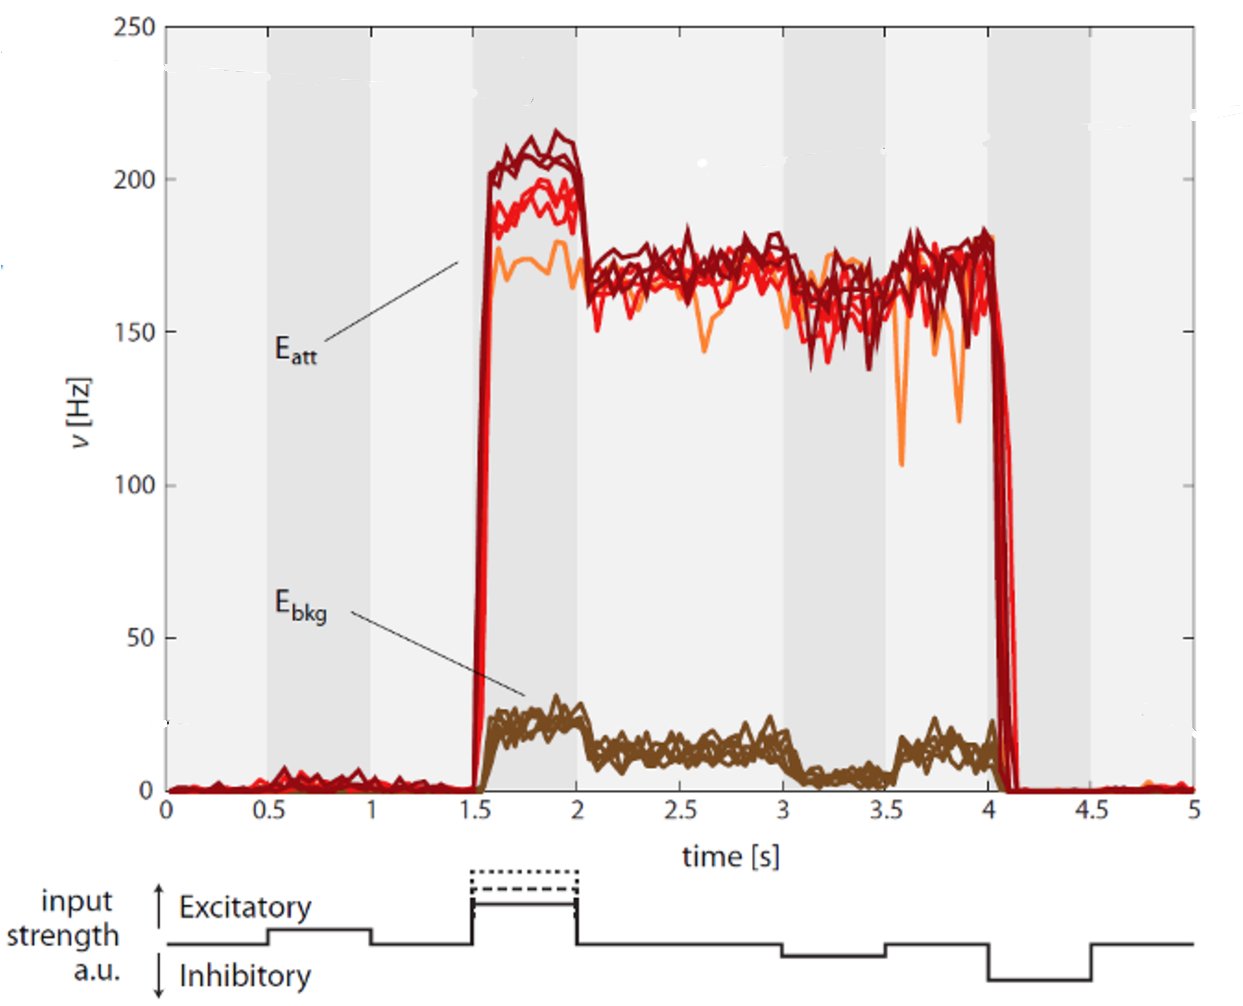
\includegraphics[width=\columnwidth]{./img/readings/Attractor_behavior.pdf}
	\caption{Point attractor network's input stimuli and neuron population firing rate \cite{giudiceRobustWorkingMemory2012}. The attractor state is obtained after a strong stimuli at 1.5s.}
	\label{fig:reading_NNbehavior}
\end{figure}